\chapter{The High Level Compiler}
\label{delite}

We begin our description of the process for compiling DSLs to FPGAs with
the high level compiler. The system diagram for this high level compiler is shown in
Figure~\ref{fig:delite-diag}.
As shown in this figure, the purpose of the high level compiler is to take
programs represented in the parallel patterns described in
Chapter~\ref{parallel-patterns} and lower them to a form which can be more easily
translated to hardware. For the purposes of this chapter, we will assume the
target DSL already has a lowering path to parallel patterns. While the
transformations described in this chapter are generally applicable to any
target hardware, we will discuss them with particular focus on their implications
when targeting FPGAs.

One of the key challenges of generating efficient custom architectures from
high level languages is in coping with arbitrarily large data structures.
Since main memory accesses are expensive and resources on the FPGA are limited,
our goal is to store a reasonably sized working set in the FPGA's local memory
for as long as possible. Ideally, we also want to hide memory transfer latencies
by overlapping communication with computation using prefetching hardware.

To this end, in this chapter we describe a method for automatically tiling parallel
patterns to improve program locality and data reuse.
Like classic loop tiling, our pattern tiling method is composed of two
transformations: strip mining and interchange.

As shown in Figure~\ref{fig:delite-diag}, the high level compiler is also responsible
for performing various well known, target-agnostic transformations like
loop fusion~\cite{rompf12optimizing,damien-thesis,vera-thesis},
loop invariant code motion, common subexpression elimination (CSE)~\cite{lms},
and data structure optimizations~\cite{rompf12optimizing}.
We refer the reader to prior work for detailed descriptions of these other transformations.

\begin{figure*}
\centering
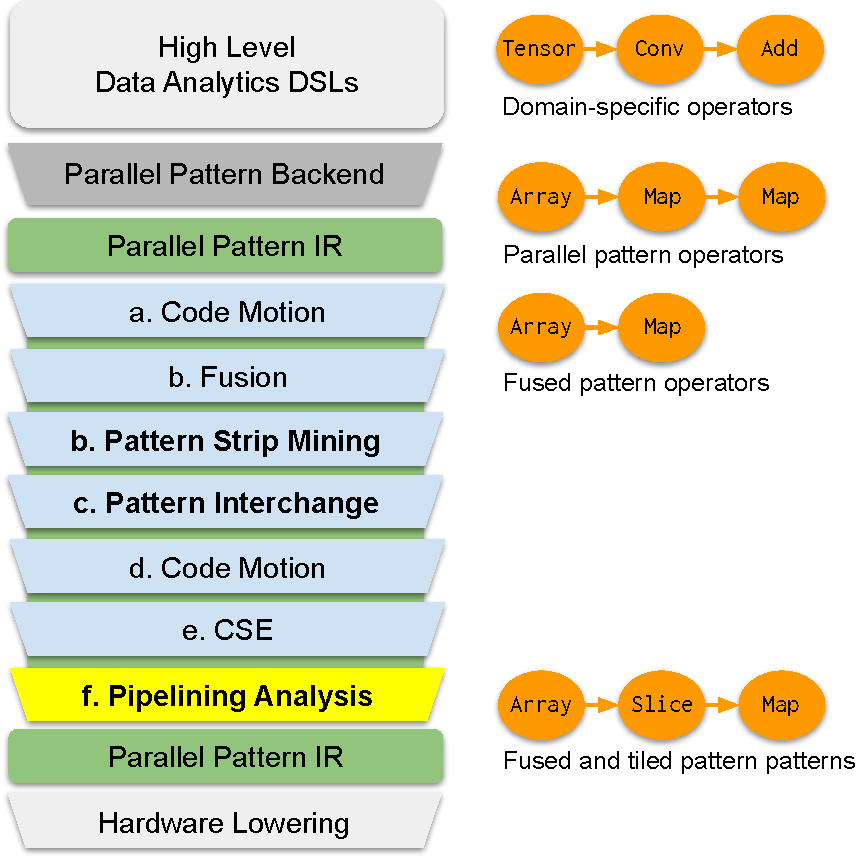
\includegraphics[width=0.8\textwidth]{3-delite/figs/delite-diag}
\caption{\label{fig:delite-diag}Block diagram of the high level compiler.
This compiler is responsible for performing various target-agnostic optimizations
on the input program, including loop fusion, loop invariant code motion, common
subexpression elimination (CSE),
and parallel pattern tiling. It also performs basic pipeline schedule analysis
and annotates this information for the lower level compiler.}
\end{figure*}

\section{Pattern Transformations}
\label{transformations}

One of the key challenges of generating efficient custom architectures from high level languages is in coping with arbitrarily large data structures. Since main memory accesses
are expensive and area is limited, our goal is to store a working set in the FPGA's local memory for as long as possible. Ideally, we also want
to hide memory transfer latencies by overlapping communication with computation using prefetching hardware blocks.
To this end, in this section we describe a method for automatically tiling parallel patterns to improve program locality and data reuse.
Like classic loop tiling, our pattern tiling method is composed of two transformations: strip mining and interchange.
We assume here that our input is a PPL representation of a program and that well known target-agnostic transformations like fusion, code motion, and struct unwrapping have already been run.

\begin{table}
\small\centering
\begin{tabular}{@{}lll@{}}
\toprule
{\bf Pattern }    & { }  & {\bf Strip Mined Pattern} \\ \midrule
{\begin{lstlisting}[mathescape=true,numbers=none,basicstyle=\fontsize{8}{8}\selectfont\tt]
T[ Map(d)(m) ]
\end{lstlisting}
} & \texttt{=} &
{\begin{lstlisting}[mathescape=true,numbers=none,basicstyle=\fontsize{8}{8}\selectfont\tt]
MultiFold(d/b)(d)(zeros(d)){ i =>
  (i, acc => Map(b)(T[m]) )
}(_)
\end{lstlisting}
} \\ \midrule
{\begin{lstlisting}[mathescape=true,numbers=none,basicstyle=\fontsize{8}{8}\selectfont\tt]
T[ MultiFold(d)(r)(z)(g)(c) ]
\end{lstlisting}
} & \texttt{=} &
{\begin{lstlisting}[mathescape=true,numbers=none,basicstyle=\fontsize{8}{8}\selectfont\tt]
MultiFold(d/b)(r)(T[z]){ i =>
  (i, acc => T[c](acc, MultiFold(b)(r)(T[z])(T[g])(T[c])) )
}(T[c])
\end{lstlisting}
} \\ \midrule
{\begin{lstlisting}[mathescape=true,numbers=none,basicstyle=\fontsize{8}{8}\selectfont\tt]
T[ GroupByFold(d)(z)(h)(c) ]
\end{lstlisting}
} & \texttt{=} &
{\begin{lstlisting}[mathescape=true,numbers=none,basicstyle=\fontsize{8}{8}\selectfont\tt]
GroupByFold(d/b)(T[z]){ i =>
  GroupByFold(b)(T[z])(T[h])(T[c])
}(T[c])
\end{lstlisting}
} \\ \midrule
{\begin{lstlisting}[mathescape=true,numbers=none,basicstyle=\fontsize{8}{8}\selectfont\tt]
T[ FlatMap(d)(f) ]
\end{lstlisting}
} & \texttt{=} &
{\begin{lstlisting}[mathescape=true,numbers=none,basicstyle=\fontsize{8}{8}\selectfont\tt]
FlatMap(d/b){i => FlatMap(b)(T[f]) }
\end{lstlisting}
} \\ \bottomrule
\end{tabular}
\caption{Strip mining transformation rules for parallel patterns defined in Figure \ref{fig:ppl-syntax}.}
\label{table:stripmining}
\end{table}


%Strip mining sequential, imperative loops is fairly straightforward.
%Due to the additional information inherent in parallel patterns, strip mining
\paragraph{Strip mining} %We first examine how parallel patterns can be strip mined.
%Simple imperative \emph{for} loops are strip mined using a single transformation rule: split the loop's domain to create a pair of nested \emph{for} loops.

%, and describes how tiles of the inner pattern should be combined into a
%representation equivalent to that created by the untiled pattern.
%The inner pattern is a transformed version of the original pattern which .
%In general, transformation rules on parallel patterns must preserve access pattern and parallelism information.
%In our intermediate representation, this necessitates that the strip mining rules  %outer loop created by strip mining a parallel pattern must itself be a parallel pattern.
%generate a set of perfectly nested parallel patterns.
The strip mining algorithm is defined here using two passes over the IR.
The first pass partitions each pattern's iteration domain \emph{d} into tiles of size \emph{b} by breaking the pattern into a pair of perfectly nested patterns.
The outer pattern operates over the strided index domain, expressed here as \emph{d/b}, while the inner pattern operates on a tile of size \emph{b}.
For the sake of brevity this notation ignores the case where \emph{b} does not perfectly divide \emph{d}.
This case is trivially solved with the addition of \emph{min} checks on the domain of the inner loop.
Table~\ref{table:stripmining} gives an overview of the rules used by transformer (denoted \emph{T}) to strip mine parallel patterns.
In addition to splitting up the domain, patterns are transformed by recursively strip mining all functions within that pattern.
Map is strip mined by reducing its domain and range and nesting it within a MultiFold. Note that the strided MultiFold writes
to each memory location only once. In this case we indicate the MultiFold's combination function as unused with an underscore.
As defined in Figure~\ref{fig:ppl-syntax}, the MultiFold, GroupByFold, and FlatMap patterns have the property that a perfectly nested form of a single instance of one of these
patterns is equivalent to a single ``flattened'' form of that same pattern. This property allows these patterns to be strip mined by
breaking them up into a set of perfectly nested patterns of the same type as the original pattern.

The second strip mining pass converts array slices and accesses with statically predictable access patterns into slices and accesses of larger, explicitly defined
array memory tiles. We define tiles which have a size statically known to fit on the FPGA using array copies.
Copies generated during strip mining can then be used to infer buffers during hardware generation.
%These buffers allow better usage of burst reads and writes from main memory and enable overlapping of compututation and communication using hardware prefetching.
Array tiles which have overlap, such as those generated from sliding windows in convolution, are marked with metadata in the IR as having some reuse factor.
Array copies with reuse have generation rules which minimize the number of redundant reads to main memory when possible.

\begin{table*}[t]
\small\centering
\begin{tabular}{@{}lll@{}}
\toprule
{\bf High Level Language}                            & {\bf PPL }       & {\bf Strip Mined PPL} \\ \midrule
{\begin{lstlisting}[numbers=none,language=Scala]
// Element-wise Map
val x: Array[Float] // length d
x.map{e => 2*e}
\end{lstlisting}}
&
{\begin{lstlisting}[numbers=none]
map(d){i => 2*x(i)}
\end{lstlisting}}
&
{\begin{lstlisting}[numbers=none]
multiFold(d/b)(d)(zeros(d)){ii =>
  xTile = x.copy(b + ii)
  (i, map(b)(b){i => 2*xTile(i) })
}(_)
\end{lstlisting}} \\ \midrule
{\begin{lstlisting}[numbers=none, language=Scala]
// Sums along matrix rows
val x: Array[Array[Float]] // m x n
x.map{ row =>
  row.fold(0){ (a,b) => a + b }
}
\end{lstlisting}}
&
{\begin{lstlisting}[numbers=none,language=PPL]
multiFold(m,n)(m)(zeros(m)){ (i,j) =>
  (i, acc => acc + x(i,j))
}{(a,b) =>
  map(n){(j) => a(j) + b(j)}
}
\end{lstlisting}}
&
{\begin{lstlisting}[numbers=none]
multiFold(m/b0,n/b1)(m)(zeros(m)){ (ii,jj) =>
  xTile = x.copy(b0 + ii, b1 + jj)
  tile = multiFold(b0,b1)(b0)(zeros(b0)){ (i,j) =>
    (i, acc => acc + xTile(i,j))
  }{(a,b) => map(b0){i => a(i) + b(i)} }
  (ii, acc => map(b0){j => acc(j) + tile(j)})
}{(a,b) =>
  multiFold(m/b0)(m)(zeros(m)){ii =>
    aTile = a.copy(b0 + ii)
    bTile = a.copy(b0 + ii)
    (ii, acc => map(b0){i => aTile(i) + bTile(i)})
  }{(a,b) => map(m){i => a(i) + b(i)}}
}
\end{lstlisting}} \\ \midrule
{\begin{lstlisting}[numbers=none]
// Simple Filter
val x: Array[Float] // length d
x.flatMap{ e =>
  if (e > 0) e else []
}
\end{lstlisting}}
&
{\begin{lstlisting}[numbers=none]
flatMap(d){i =>
  if (x(i) > 0) x(i) else []
}
\end{lstlisting}}
&
{\begin{lstlisting}[numbers=none]
flatMap(d/b)(1){ii =>
  eTile = x.copy(b + ii)
  flatMap(b){i =>
    if (eTile(i) > 0) eTile(i) else []
}}
\end{lstlisting}} \\ \midrule
{\begin{lstlisting}[numbers=none]
// Histogram Calculation
val x: Array[Float] // length d
x.groupByFold(0){ r =>
  (r/10, 1)
}{ (a,b) => a + b }
\end{lstlisting}}
&
{\begin{lstlisting}[numbers=none]
groupByFold(d)(0){i =>
  (x(i)/10, 1)
}{(a,b) => a + b }
\end{lstlisting}}
&
{\begin{lstlisting}[numbers=none]
groupByFold(d/b)(0){ii =>
  xTile = x.copy(b + ii)
  groupByFold(b)(0){i =>
    (xTile(i)/10, 1)
  }{(a,b) => a + b}
}{(a,b) => a + b}
\end{lstlisting}} \\ \bottomrule
\end{tabular}
\caption{Examples of the parallel pattern strip mining transformation on Map, MultiFold, FlatMap, and GroupByFold}
\label{table:stripmine-examples}
\end{table*}

\begin{table*}[t]
\centering\small
\begin{tabular}{@{}lll@{}}
\toprule
{\bf High Level Language}                            & {\bf Strip Mined PPL }       & {\bf Interchanged PPL} \\ \midrule
{\begin{lstlisting}[numbers=none]
// Matrix Multiplication
x: Array[Array[Float]] // m x p
y: Array[Array[Float]] // p x n
z = x.map{row =>
  y.map{col =>
    row.zipWith(col){(a,b) =>
      a * b
    }.sum
  }
}
\end{lstlisting}}
&
{\begin{lstlisting}[numbers=none]
multiFold(m/b0,n/b1)(m,n)(zeros(m,n)){(ii,jj) =>
(*@\color{vbgray}{\vrule}@*)  ((ii,jj), zTile =>
(*@\color{vbgray}{\vrule}@*)  (*@\color{vbgray}{\vrule}@*)  map(b0,b1){(i,j) =>
(*@\color{vbgray}{\vrule}@*)  (*@\color{vbgray}{\vrule}@*)  (*@\color{vbgray}{\vrule}@*)  tile = multiFold(p/b2)(1)(0){ kk =>
(*@\color{vbgray}{\vrule}@*)  (*@\color{vbgray}{\vrule}@*)  (*@\color{vbgray}{\vrule}@*)  (*@\color{vbgray}{\vrule}@*)  xTile = x.copy(b0 + ii, b2 + kk)
(*@\color{vbgray}{\vrule}@*)  (*@\color{vbgray}{\vrule}@*)  (*@\color{vbgray}{\vrule}@*)  (*@\color{vbgray}{\vrule}@*)  yTile = y.copy(b2 + kk, b1 + jj)
(*@\color{vbgray}{\vrule}@*)  (*@\color{vbgray}{\vrule}@*)  (*@\color{vbgray}{\vrule}@*)  (*@\color{vbgray}{\vrule}@*)  dprod = fold(b2)(0){ k =>
(*@\color{vbgray}{\vrule}@*)  (*@\color{vbgray}{\vrule}@*)  (*@\color{vbgray}{\vrule}@*)  (*@\color{vbgray}{\vrule}@*)  (*@\color{vbgray}{\vrule}@*)  acc => acc + xTile(i,k) * yTile(k,j)
(*@\color{vbgray}{\vrule}@*)  (*@\color{vbgray}{\vrule}@*)  (*@\color{vbgray}{\vrule}@*)  (*@\color{vbgray}{\vrule}@*)  }{(a,b) => a + b})
(*@\color{vbgray}{\vrule}@*)  (*@\color{vbgray}{\vrule}@*)  (*@\color{vbgray}{\vrule}@*)  (*@\color{vbgray}{\vrule}@*)  (0, elemTile => elemTile + dprod)
(*@\color{vbgray}{\vrule}@*)  (*@\color{vbgray}{\vrule}@*)  (*@\color{vbgray}{\vrule}@*)  }{(a,b) => a + b}
(*@\color{vbgray}{\vrule}@*)  (*@\color{vbgray}{\vrule}@*)  (*@\color{vbgray}{\vrule}@*)  zTile(i,j) + tile
(*@\color{vbgray}{\vrule}@*)  })
}(_)
\end{lstlisting}}
&
{\begin{lstlisting}[numbers=none]
multiFold(m/b0,n/b1)(m,n)(zeros(m,n)){(ii,jj) =>
(*@\color{vbgray}{\vrule}@*)  tile = multiFold(p/b2)(b0,b1)(...){kk =>
(*@\color{vbgray}{\vrule}@*)  (*@\color{vbgray}{\vrule}@*)  xTile = x.copy(b0 + ii, b2 + kk)
(*@\color{vbgray}{\vrule}@*)  (*@\color{vbgray}{\vrule}@*)  yTile = y.copy(b2 + kk, b1 + jj)
(*@\color{vbgray}{\vrule}@*)  (*@\color{vbgray}{\vrule}@*)  (0, elemTile =>
(*@\color{vbgray}{\vrule}@*)  (*@\color{vbgray}{\vrule}@*)  (*@\color{vbgray}{\vrule}@*)  map(b0,b1){(i,j) =>
(*@\color{vbgray}{\vrule}@*)  (*@\color{vbgray}{\vrule}@*)  (*@\color{vbgray}{\vrule}@*)  (*@\color{vbgray}{\vrule}@*)  dprod = fold(b2)(0){ k =>
(*@\color{vbgray}{\vrule}@*)  (*@\color{vbgray}{\vrule}@*)  (*@\color{vbgray}{\vrule}@*)  (*@\color{vbgray}{\vrule}@*)  (*@\color{vbgray}{\vrule}@*)  acc => acc + xTile(i,j) * yTile(j,k)
(*@\color{vbgray}{\vrule}@*)  (*@\color{vbgray}{\vrule}@*)  (*@\color{vbgray}{\vrule}@*)  (*@\color{vbgray}{\vrule}@*)  }{(a,b) => a + b}
(*@\color{vbgray}{\vrule}@*)  (*@\color{vbgray}{\vrule}@*)  (*@\color{vbgray}{\vrule}@*)  (*@\color{vbgray}{\vrule}@*)  elemTile(i,j) + dprod
(*@\color{vbgray}{\vrule}@*)  (*@\color{vbgray}{\vrule}@*)  })
(*@\color{vbgray}{\vrule}@*)  }{(a,b) =>
(*@\color{vbgray}{\vrule}@*)  (*@\color{vbgray}{\vrule}@*)  map(b0,b1){(i,j) => a(i,j) + b(i,j)
(*@\color{vbgray}{\vrule}@*)  }
(*@\color{vbgray}{\vrule}@*)  ((ii,jj), zTile =>
(*@\color{vbgray}{\vrule}@*)  (*@\color{vbgray}{\vrule}@*)  map(b0,b1){(i,j) => zTile(i,j) + tile(i,j)}
(*@\color{vbgray}{\vrule}@*)  })
}(_)
\end{lstlisting}} \\ \bottomrule
\end{tabular}
\caption{Example of the pattern interchange transformation applied to matrix multiplication.}
\label{table:interchange-examples}
\end{table*}


Table~\ref{table:stripmine-examples} demonstrates how our rules can be used to strip mine a set of simple data parallel operations.
We use the \emph{copy} infix function on arrays to designate array copies in these examples, using similar syntax as array \emph{slice}.
We assume in these examples that common subexpression elimination (CSE) and code motion transformation passes have been run after strip mining to eliminate duplicate copies and to
move array tiles out of the innermost patterns. In these examples, strip mining creates tiled copies of input collections that
we can later directly use to infer read buffers.

% \begin{table*}[t]\small\centering
% \begin{tabular}{@{}lll@{}}
% \toprule
% {\bf Nested Pattern }    & { }  & {\bf Interchanged Patterns} \\ \midrule
% {\begin{lstlisting}[mathescape=true,numbers=none]
% Map(d$_0$){i =>
%   MultiFold(d$_1$/b)(1)(z)(f)(c)
% }
% \end{lstlisting}
% } & \texttt{=>} &
% {\begin{lstlisting}[mathescape=true,numbers=none]
% MultiFold(d$_1$/b)(1)(Map(d$_0$)(z))(
%   (0, acc => Map(d$_0$){i => c(acc(i), f._2) })
% ){(a,b) => Map(d$_0$){i => c(a(i), b(i)) }}
% \end{lstlisting}
% } \\ \midrule
% {\begin{lstlisting}[mathescape=true,numbers=none]
% MultiFold(d$_0$)(d$_1$)(z)(
%   x = MultiFold(d$_1$/b)(d$_1$)(zeros(d$_1$))(f)(_)
%   (0, acc => MultiFold(d$_1$/b)(d$_1$)(zeros(d$_1$))(c(acc,x))(_))
% ){(a,b) =>
%   MultiFold(d$_1$/b)(d$_1$)(zeros(d$_1$))(c(a,b))(_)
% }
% \end{lstlisting}
% } & \texttt{=>} &
% {\begin{lstlisting}[mathescape=true,numbers=none]
% MultiFold(d$_1$/b)(d$_1$)(zeros(d$_1$))(
%   (0, acc => MultiFold(d$_0$)(1)(z)(f)(c) )
% )(_)
% \end{lstlisting}
% } \\ \bottomrule
% \end{tabular}
% \caption{Interchange transformation rules for pattern tiling.}
% \label{table:interchange}
% \end{table*}



\paragraph{Pattern interchange}
Given an intermediate representation with strip mined nested parallel patterns, we now need to interchange patterns to increase the reuse
of newly created data tiles. This can be achieved by moving strided patterns out of unstrided patterns. However, as with imperative loops,
it is not sound to arbitrarily change the order of nested parallel patterns.
We use two rules for pattern interchange adapted from a previously established \emph{Collect}-\emph{Reduce} reordering rule for computation on clusters~\cite{brown16clusters}.
These rules both match on the special case of MultiFold where every iteration updates the entire accumulator, which we refer to here as a \emph{fold}.
The first interchange rule defines how to move a scalar, strided \emph{fold} out of an unstrided Map, transforming the nested loop into a strided \emph{fold} of a Map.
Note that this also changes the combination function of the \emph{fold} into a Map.
The second rule is the inverse of the first, allowing us to reorder a strided MultiFold with no reduction function (i.e. the outer pattern of a tiled Map)
out of an unstrided \emph{fold}. This creates a strided MultiFold of a scalar \emph{fold}. We apply these two rules whenever possible to increase the reuse
of tiled inputs.
%The first rule defines how to reorder a Map out of

%ur pattern interchange rules are defined only on specific cases of perfectly nested patterns. These rules are given in Table~\ref{table:interchange}.
%Our rules define how to move
%a strided Fold out of an unstrided Map, creating a
%and a strided Map out of an unstrided Fold.


Imperfectly nested parallel patterns commonly occur either due to the way the original user program was structured or
as a result of aggressive vertical fusion run prior to tiling.
Interchange on imperfectly nested patterns requires splitting patterns into perfectly nested sections. However, splitting and reordering trades
temporal locality of intermediate values for increased reuse of data tiles. In hardware, this can involve creating more main memory
reads or larger on-chip buffers for intermediate results so that less reads need to be done for input and output data. This tradeoff between memory reads and
increased buffer usage requires more complex cost modeling.
We use a simple heuristic to determine whether to split fused loops: we split and interchange patterns only when
the intermediate result created after splitting and interchanging is statically known to fit on the FPGA. This handles the simple case
where the FPGA has unused on-chip buffers and allocating more on-chip memory guarantees a decrease in the number of main memory reads.
Future work will examine ways to statically model the tradeoff between main memory accesses and local buffers near 100\% on-chip memory utilization.


Table~\ref{table:interchange-examples} shows a simple example of the application of our pattern interchange rules on matrix multiplication.
We assume here that code motion has been run again after pattern interchange has completed.
In matrix multiplication, we interchange the perfectly nested strided MultiFold and the unstrided Map.
This ordering increases the reuse of the copied tile of matrix \emph{y} and changes the scalar reduction into a tile-wise reduction.
Note that the partial result calculation and the inner reduction can now be vertically fused.



\begin{figure*}\small\centering
%\begin{minipage}[b]{.4\textwidth}
\hspace{-0.105\textwidth}
\centering\begin{tabular}{cm{0.45\textwidth}m{0.01\textwidth}m{0.44\textwidth}}
{} &
{\begin{lstlisting}
(sums,counts) = multiFold(n/b0)((k,d),k)(...){ii =>
(*@\color{vbgray}{\vrule}@*)  pt1Tile = points.copy(b0 + ii, *)
(*@\color{vbgray}{\vrule}@*)  multiFold(b0)((k,d),k)(zeros(1,d),0){ i =>
(*@\color{vbgray}{\vrule}@*)  (*@\color{vbgray}{\vrule}@*)  pt1 = pt1Tile.slice(i, *)
(*@\color{vbgray}{\vrule}@*)  (*@\color{vbgray}{\vrule}@*)  minDistWithIndex = multiFold(k/b1)(1)((max, -1)){ jj =>
(*@\color{vbgray}{\vrule}@*)  (*@\color{vbgray}{\vrule}@*)  (*@\color{vbgray}{\vrule}@*)  pt2Tile = centroids.copy(b1 + jj, *)
(*@\color{vbgray}{\vrule}@*)  (*@\color{vbgray}{\vrule}@*)  (*@\color{vbgray}{\vrule}@*)  minIndTile = fold(b1)((max,-1)){ j =>
(*@\color{vbgray}{\vrule}@*)  (*@\color{vbgray}{\vrule}@*)  (*@\color{vbgray}{\vrule}@*)  (*@\color{vbgray}{\vrule}@*)  pt2 = pt2Tile.slice(j, *)
(*@\color{vbgray}{\vrule}@*)  (*@\color{vbgray}{\vrule}@*)  (*@\color{vbgray}{\vrule}@*)  (*@\color{vbgray}{\vrule}@*)  dist = distance(pt1, pt2)
(*@\color{vbgray}{\vrule}@*)  (*@\color{vbgray}{\vrule}@*)  (*@\color{vbgray}{\vrule}@*)  (*@\color{vbgray}{\vrule}@*)  acc => if (acc._1 < dist) acc else (dist, j+jj)
(*@\color{vbgray}{\vrule}@*)  (*@\color{vbgray}{\vrule}@*)  (*@\color{vbgray}{\vrule}@*)  }{ (a,b) => if (a._1 < b._1) a else b }
(*@\color{vbgray}{\vrule}@*)  (*@\color{vbgray}{\vrule}@*)  (*@\color{vbgray}{\vrule}@*)
(*@\color{vbgray}{\vrule}@*)  (*@\color{vbgray}{\vrule}@*)  (*@\color{vbgray}{\vrule}@*)  (0, acc =>
(*@\color{vbgray}{\vrule}@*)  (*@\color{vbgray}{\vrule}@*)  (*@\color{vbgray}{\vrule}@*)    if (acc._1 < minIndTile._1) acc else minIndTile)
(*@\color{vbgray}{\vrule}@*)  (*@\color{vbgray}{\vrule}@*)  }{(a,b) =>
(*@\color{vbgray}{\vrule}@*)  (*@\color{vbgray}{\vrule}@*)    if (a._1 < b._1) a else b
(*@\color{vbgray}{\vrule}@*)  (*@\color{vbgray}{\vrule}@*)  }
(*@\color{vbgray}{\vrule}@*)  (*@\color{vbgray}{\vrule}@*)
(*@\color{vbgray}{\vrule}@*)  (*@\color{vbgray}{\vrule}@*)
(*@\color{vbgray}{\vrule}@*)  (*@\color{vbgray}{\vrule}@*)  minDistIndex = minDistWithIndex._2
(*@\color{vbgray}{\vrule}@*)  (*@\color{vbgray}{\vrule}@*)  sumFunc = ... // Fig 4: lines 17-20
(*@\color{vbgray}{\vrule}@*)  (*@\color{vbgray}{\vrule}@*)  countFunc = ... // Fig 4: line 21
(*@\color{vbgray}{\vrule}@*)  (*@\color{vbgray}{\vrule}@*)  (sumFunc, countFunc)
(*@\color{vbgray}{\vrule}@*)  }{(a,b) => ... /* Tiled combination function */ }
(*@\color{vbgray}{\vrule}@*)  (0, acc => ... /* Tiled combination function */ )
}{(a,b) => ... /* Tiled combination function */ }

newCentroids = multiFold(k/b1,d)(k,d)(...){ (ii,jj) =>
(*@\color{vbgray}{\vrule}@*)  sumsBlk = sums.copy(b1 + ii, *)
(*@\color{vbgray}{\vrule}@*)  countsBlk = counts.copy(b1 + ii)
(*@\color{vbgray}{\vrule}@*)  (ii, acc => map(k,d){ (i,j) =>
(*@\color{vbgray}{\vrule}@*)    sumsBlk(i,j) / countsBlk(i)
(*@\color{vbgray}{\vrule}@*)  })
}
\end{lstlisting}} & \hfill &
%\end{minipage} \hfill
%\begin{minipage}[b]{.4\textwidth}
{\begin{lstlisting}
(sums,counts) = multiFold(n/b0)((k,d),k)(...){ ii =>
(*@\color{vbgray}{\vrule}@*)  pt1Tile = points.copy(b0 + ii, *)
(*@\color{vbgray}{\vrule}@*)  minDistWithInds = multiFold(k/b1)(b1)(map(b1)((max, -1))){ jj =>
(*@\color{vbgray}{\vrule}@*)  (*@\color{vbgray}{\vrule}@*)  pt2Tile = centroids.copy(b1 + jj, *)
(*@\color{vbgray}{\vrule}@*)  (*@\color{vbgray}{\vrule}@*)  minIndsTile = map(b0){ i =>
(*@\color{vbgray}{\vrule}@*)  (*@\color{vbgray}{\vrule}@*)  (*@\color{vbgray}{\vrule}@*)  pt1 = pt1Tile.slice(i, *)
(*@\color{vbgray}{\vrule}@*)  (*@\color{vbgray}{\vrule}@*)  (*@\color{vbgray}{\vrule}@*)  minIndTile = fold(b1)((max,-1)){ j =>
(*@\color{vbgray}{\vrule}@*)  (*@\color{vbgray}{\vrule}@*)  (*@\color{vbgray}{\vrule}@*)  (*@\color{vbgray}{\vrule}@*)  pt2 = pt2Tile.slice(j, *)
(*@\color{vbgray}{\vrule}@*)  (*@\color{vbgray}{\vrule}@*)  (*@\color{vbgray}{\vrule}@*)  (*@\color{vbgray}{\vrule}@*)  dist = distance(pt1, pt2)
(*@\color{vbgray}{\vrule}@*)  (*@\color{vbgray}{\vrule}@*)  (*@\color{vbgray}{\vrule}@*)  (*@\color{vbgray}{\vrule}@*)  acc => if (acc._1 < dist) acc else (dist, j+jj)
(*@\color{vbgray}{\vrule}@*)  (*@\color{vbgray}{\vrule}@*)  (*@\color{vbgray}{\vrule}@*)  }{ (a,b) => if (a._1 < b._1) a else b }
(*@\color{vbgray}{\vrule}@*)  (*@\color{vbgray}{\vrule}@*)  }
(*@\color{vbgray}{\vrule}@*)  (*@\color{vbgray}{\vrule}@*)  (0, acc => map(b0){ i =>
(*@\color{vbgray}{\vrule}@*)  (*@\color{vbgray}{\vrule}@*)    if (acc(i)._1 < minIndsTile(i)._1) acc else minIndsTile(i) })
(*@\color{vbgray}{\vrule}@*)  }{(a,b) =>
(*@\color{vbgray}{\vrule}@*)    map(b0){i => if (a(i)._1 < b(i)._1) a(i) else b(i) }
(*@\color{vbgray}{\vrule}@*)  }
(*@\color{vbgray}{\vrule}@*)  multiFold(b0)(k,d)(zeros(k,d)){ i =>
(*@\color{vbgray}{\vrule}@*)  (*@\color{vbgray}{\vrule}@*)  pt1 = pt1Tile.slice(i, *)
(*@\color{vbgray}{\vrule}@*)  (*@\color{vbgray}{\vrule}@*)  minDistIndex = minDistWithInds(i)._2
(*@\color{vbgray}{\vrule}@*)  (*@\color{vbgray}{\vrule}@*)  sumFunc = ... // Fig 4: lines 17-20
(*@\color{vbgray}{\vrule}@*)  (*@\color{vbgray}{\vrule}@*)  countFunc = ... // Fig 4: line 21
(*@\color{vbgray}{\vrule}@*)  (*@\color{vbgray}{\vrule}@*)  (sumFunc, countFunc)
(*@\color{vbgray}{\vrule}@*)  }{(a,b) => ... /* Tiled combination function */ }
(*@\color{vbgray}{\vrule}@*)  (0, acc => ... /* Tiled combination function */ )
}{(a,b) => ... /* Tiled combination function */ }

newCentroids = multiFold(k/b1,d)(k,d)(...){ (ii,jj) =>
(*@\color{vbgray}{\vrule}@*)  sumsBlk = sums.copy(b1 + ii, *)
(*@\color{vbgray}{\vrule}@*)  countsBlk = counts.copy(b1 + ii)
(*@\color{vbgray}{\vrule}@*)  (ii, acc => map(k,d){ (i,j) =>
(*@\color{vbgray}{\vrule}@*)    sumsBlk(i,j) / countsBlk(i)
(*@\color{vbgray}{\vrule}@*)  })
}
\end{lstlisting}}
\end{tabular}

\vspace{-0.2in}\begin{tabular}{cc}
{\parbox{0.45\textwidth}{\centering{(a) Strip mined $k$-means in PPL.}}} &
{\parbox{0.5\textwidth}{\centering{(b) Pattern Interchanged $k$-means in PPL.}}}
\end{tabular}

%\vspace{-0.045\textwidth}
\hspace{-0.180\textwidth}
\centering\begin{tabular}{cm{0.45\textwidth}m{0.01\textwidth}m{0.44\textwidth}}
{} &
{\begin{lstlisting}[numbers=none,language=Pseudo]
1     For each tile of b0 points:
2     (*@\color{vbgray}{\vrule}@*)  Copy the points tile into local memory
3 - 4 (*@\color{vbgray}{\vrule}@*)  (*@\textbf{\color{blue}{For each point \emph{pt1} in the points tile}}@*):
5     (*@\color{vbgray}{\vrule}@*)  (*@\color{vbgray}{\vrule}@*)  (*@\textbf{\color{red}{For each tile of b1 centroids}}@*):
6     (*@\color{vbgray}{\vrule}@*)  (*@\color{vbgray}{\vrule}@*)  (*@\color{vbgray}{\vrule}@*)  Copy the centroids tile into local memory
7 - 8 (*@\color{vbgray}{\vrule}@*)  (*@\color{vbgray}{\vrule}@*)  (*@\color{vbgray}{\vrule}@*)  For each centroid (*@\emph{pt2}@*) in the centroids tile:
9     (*@\color{vbgray}{\vrule}@*)  (*@\color{vbgray}{\vrule}@*)  (*@\color{vbgray}{\vrule}@*)  (*@\color{vbgray}{\vrule}@*)  Compute distance between (*@\emph{pt1}@*) and (*@\emph{pt2}@*)
10-11 (*@\color{vbgray}{\vrule}@*)  (*@\color{vbgray}{\vrule}@*)  (*@\color{vbgray}{\vrule}@*)  (*@\color{vbgray}{\vrule}@*)  Keep the closest (index,distance) pair
      (*@\color{vbgray}{\vrule}@*)  (*@\color{vbgray}{\vrule}@*)  (*@\color{vbgray}{\vrule}@*)  End
13-16 (*@\color{vbgray}{\vrule}@*)  (*@\color{vbgray}{\vrule}@*)  (*@\color{vbgray}{\vrule}@*)  Keep the closest pair across tiles
      (*@\color{vbgray}{\vrule}@*)  (*@\color{vbgray}{\vrule}@*)  End
20    (*@\color{vbgray}{\vrule}@*)  (*@\color{vbgray}{\vrule}@*)  Extract the index of the closest centroid
21    (*@\color{vbgray}{\vrule}@*)  (*@\color{vbgray}{\vrule}@*)  Add (*@\emph{pt1}@*) to row minDistIndex
22    (*@\color{vbgray}{\vrule}@*)  (*@\color{vbgray}{\vrule}@*)  Increment count at minDistIndex
24    (*@\color{vbgray}{\vrule}@*)  (*@\color{vbgray}{\vrule}@*)  Add point and count sums across tiles
      (*@\color{vbgray}{\vrule}@*)  End
25-26 (*@\color{vbgray}{\vrule}@*)  Add point and count sums across tiles
      End

28    For each tile of b1 point sums and counts:
29    (*@\color{vbgray}{\vrule}@*)  Copy the point sums tile into local memory
30    (*@\color{vbgray}{\vrule}@*)  Copy the point counts tile into local memory
31-32 (*@\color{vbgray}{\vrule}@*)  Compute each new centroid as sums(i) / count(i)
      End
\end{lstlisting}} & \hfill &
%\end{minipage} \hfill
%\begin{minipage}[b]{.4\textwidth}
{\begin{lstlisting}[numbers=none,language=Pseudo]
1     For each tile of b0 points:
2     (*@\color{vbgray}{\vrule}@*)  Copy the points tile into local memory
3     (*@\color{vbgray}{\vrule}@*)  (*@\color{red}{\textbf{For each tile of b1 centroids}}@*):
4     (*@\color{vbgray}{\vrule}@*)  (*@\color{vbgray}{\vrule}@*)  Copy the centroids tile into local memory
5 - 6 (*@\color{vbgray}{\vrule}@*)  (*@\color{vbgray}{\vrule}@*)  (*@\color{blue}{\textbf{For each point \emph{pt1} in the points tile}}@*):
7 - 8 (*@\color{vbgray}{\vrule}@*)  (*@\color{vbgray}{\vrule}@*)  (*@\color{vbgray}{\vrule}@*)  For each centroid (*@\emph{pt2}@*) in the centroids tile:
9     (*@\color{vbgray}{\vrule}@*)  (*@\color{vbgray}{\vrule}@*)  (*@\color{vbgray}{\vrule}@*)  (*@\color{vbgray}{\vrule}@*)  Compute distance between (*@\emph{pt1}@*) and (*@\emph{pt2}@*)
10-11 (*@\color{vbgray}{\vrule}@*)  (*@\color{vbgray}{\vrule}@*)  (*@\color{vbgray}{\vrule}@*)  (*@\color{vbgray}{\vrule}@*)  Keep the closest (index,distance) pair
      (*@\color{vbgray}{\vrule}@*)  (*@\color{vbgray}{\vrule}@*)  (*@\color{vbgray}{\vrule}@*)  End
      (*@\color{vbgray}{\vrule}@*)  (*@\color{vbgray}{\vrule}@*)  End
13-16 (*@\color{vbgray}{\vrule}@*)  (*@\color{vbgray}{\vrule}@*)  For each point: keep the closest pair across tiles
      (*@\color{vbgray}{\vrule}@*)  End
18-19 (*@\color{vbgray}{\vrule}@*)  (*@\color{blue}{\textbf{For each point \emph{pt1} in points tile}}@*):
20    (*@\color{vbgray}{\vrule}@*)  (*@\color{vbgray}{\vrule}@*)  Extract the index of the closest centroid
21    (*@\color{vbgray}{\vrule}@*)  (*@\color{vbgray}{\vrule}@*)  Add (*@\emph{pt1}@*) to row minDistIndex
22    (*@\color{vbgray}{\vrule}@*)  (*@\color{vbgray}{\vrule}@*)  Increment count at minDistIndex
24    (*@\color{vbgray}{\vrule}@*)  (*@\color{vbgray}{\vrule}@*)  Add point and count sums across tiles
      (*@\color{vbgray}{\vrule}@*)  End
25-26 (*@\color{vbgray}{\vrule}@*)  Add point and count sums across tiles
      End

28    For each tile of b1 point sums and counts:
29    (*@\color{vbgray}{\vrule}@*)  Copy the point sums tile into local memory
30    (*@\color{vbgray}{\vrule}@*)  Copy the point counts tile into local memory
31-32 (*@\color{vbgray}{\vrule}@*)  Compute each new centroid as sum / count
      End
\end{lstlisting}}
\end{tabular}


\vspace{-0.2in}\begin{tabular}{cc}
{\parbox{0.45\textwidth}{\centering{(c) Pseudocode description of strip mined $k$-means.}}} &
{\parbox{0.5\textwidth}{\centering{(d) Pseudocode description of pattern interchanged $k$-means.}}}
\end{tabular}

\vspace{0.1in}
\footnotesize{\begin{tabular}{|l|cc|cc|cc|}

\noalign{\hrule height 1.5pt}
\multicolumn{1}{|c|}{} & \multicolumn{2}{c|}{\bf Fused} & \multicolumn{2}{c|}{\bf Strip Mined}  & \multicolumn{2}{c|}{\bf Interchanged} \\
& Main Memory Reads & On-Chip Storage & Main Memory Reads & On-Chip Storage & Main Memory Reads & On-Chip Storage \\ \hline
\emph{points} & $n \times d$ & $d$ & $n \times d$ & $b_0 \times d$ & $n \times d$ & $b_0 \times d$ \\ \hline
\emph{centroids} & $n \times k \times d$ & $d$ & $n \times k \times d$ & $b_1 \times d$ & $(n/b_0) \times k \times d$ & $b_1 \times d$ \\ \hline
\emph{minDistWithIndex} & $0$ & $2$ & $0$ & $2$ & $0$ & $2 \times b_0$ \\
\noalign{\hrule height 1.5pt}
\end{tabular}}

\small
\vspace{0.1in}\centering{(e) Minimum number of words read from main memory and on-chip storage for data structures within $k$-means clustering after each IR transformation.}

%\end{minipage}
%\vspace{-0.1in}
%\centering\includegraphics[width=2.2in]{figs/tiledKmeans.pdf}
\caption{Full tiling example for $k$-means clustering, starting from the fused representation in Figure \ref{fig:kmeans-fused}, using tile sizes of \emph{b$_0$} and \emph{b$_1$} for the number of points $n$ and the number of clusters $k$. The number of features $d$ is not tiled in this example.}
\label{fig:kmeans-example}
\end{figure*}


\paragraph{Discussion}
The rules we outline here for automatic tiling of parallel patterns are target-agnostic. However, tile copies should only be made explicit
for devices with scratchpad memory. Architectures with hierarchical memory systems effectively maintain views of subsections of memory
automatically through caching, making explicit copies on these architectures a waste of both compute cycles and memory.

%We currently only support tiling of simple affine access and slicing patterns, where each index is either constant or of the form \emph{i + c},
%where \emph{i} is some parallel pattern index and \emph{c} is loop invariant. While this is only a subset of all affine accesses,
%these accesses are extremely common access pattern in the data analytics domain.
We currently require the user to explicitly specify tile sizes for all dimensions which require tiling. In future work, tile sizes for all pattern
dimensions will instead be determined by the compiler through automated tile size selection using modeling and design space exploration.

\paragraph{Example} We conclude this section with a complete example of tiling the $k$-means clustering algorithm, starting from the fused representation shown in Figure~\ref{fig:kmeans-fused}. We assume here that we wish
to tile the number of input points, \emph{n}, with tile size \emph{b$_0$} and the number of clusters, \emph{k}, with tile size \emph{b$_1$} but not the number of dimensions, \emph{d}. This is representative of machine learning
classification problems where the number of input points and number of labels is large, but the number of features for each point is relatively small.

Figure~\ref{fig:kmeans-example} gives a comparison of the $k$-means clustering algorithm after strip mining and after pattern interchange. During strip mining, we create
tiles for both the \emph{points} and \emph{centroids} arrays, which helps us to take advantage of main memory burst reads. However, in the strip mined version, we still fully
calculate the closest centroid for each point. This requires the entirety of \emph{centroids} to be read for each point. We increase the reuse of each tile of \emph{centroids} by first splitting
the calculation of the closest centroid label from the MultiFold (Figure~\ref{fig:kmeans-example}a. line~5). The iteration over the centroids tile is then perfectly nested within the iteration over the points. Interchanging these two iterations allows us to reuse the centroids tile across points, thus decreasing the total number of main memory reads for this array by a factor of \emph{b$_0$}. This decrease comes
at the expense of changing the intermediate (distance, label) pair for a single point to a set of intermediate pairs for an entire tile of \emph{points}. Since the created intermediate result
has size 2\emph{b$_0$}, we statically determine that this is an advantageous tradeoff and use the split and interchanged form of the algorithm.

\section{Evaluation}
\label{delite-evaluation}

\definecolor{bar1}{HTML}{5381BB}
\definecolor{bar2}{HTML}{BF4D4D}
\definecolor{bar3}{HTML}{9ABC5F}
\definecolor{bar4}{HTML}{8163A0}

We conclude this chapter by comparing the performance and
area utilization of generated FPGA implementations of a set of data analytic benchmarks.
We assume here that the remainder of the compiler framework is in place, and focus our evaluation on the improvements that our tiling transformations and
coarse-grained pipeline scheduling provide relative to
generated hardware designs that do not have these features.

\begin{table}
\centering\footnotesize
\hspace{-0.022\textwidth}\begin{tabular}{lll}
\toprule

{\bf Benchmark} & {\bf Description} & {\bf Collections Ops}\\ \midrule
outerprod & Vector outer product & \emph{map}\\ \midrule
sumrows & Summation through matrix rows & \emph{map, reduce}\\ \midrule
gemm & Matrix multiplication & \emph{map, reduce}\\ \midrule
tpchq6 & TPC-H Query 6 & \emph{filter, reduce}\\ \midrule
%sobel & Sobel edge detection & Map \\ \midrule
logreg & Logistic regression & \emph{map, reduce}\\ \midrule
gda & Gaussian discriminant analysis & \emph{map, filter, reduce}\\ \midrule
blackscholes & Black-Scholes option pricing & \emph{map}\\ \midrule
kmeans & $k$-means clustering & \emph{map, groupBy, reduce}\\ \bottomrule
%knn & k Nearest Neighbors & MultiFold, Map, GroupByFold \\ \bottomrule
\end{tabular}

\caption{Evaluation benchmarks with major collections operations used by
Scala implementation.}
\label{table:benchmarks}
\end{table}

\subsection{Methodology}
The benchmarks used in our evaluation are summarized in Table~\ref{table:benchmarks}.
We choose to study vector outer product, matrix row summation, and matrix multiplication as these exemplify many commonly occurring access patterns in the machine learning domain.
TPC-H Query 6 is a data querying application which reads a table of purchase records, filtering all
records which match a given predicate. It then computes the sum of a product of two columns in the filtered records.
Logistic regression is a binary discriminative classification algorithm that uses the sigmoid function in the calculation of predictions.
Gaussian discriminant analysis (GDA) is a classification algorithm which models the distribution of each class as a multivariate Gaussian.
Black-Scholes is a financial analytics application for option pricing.
$k$-means clustering groups a set of input points by iteratively calculating the $k$ best cluster centroids.
In our implementations, all of these benchmarks operate on single precision, floating point data.

We implement our transformation and hardware generation steps in an existing compiler framework called Delite~\cite{delite-tecs14}.
We write each of our benchmark applications in OptiML~\cite{optiml}, a high level, domain specific language embedded in Scala for machine learning which can be compiled by the Delite compiler.
We then compile each of these applications with the modified compiler.
During compilation, applications are compiled into their PPL intermediate representations.
The compiler then performs the tiling transformations and pipeline scheduling.
%These VHDL descriptions are compiled to a final FPGA configuration bitstream by Altera synthesis tools.
%Delite also links in C libraries for handling file reading, transferring data between CPU DRAM and FPGA DRAM, and configuring the FPGA with the generated bitstream.
We measure the running times of these designs starting after input data has
been copied to the FPGA's DRAM and ending when the hardware design reports completion.
Final running times were calculated as an arithmetic mean of five individual run times to account for small runtime variations in main memory accesses and the device driver stack.

We run each generated design on an Altera Stratix V FPGA on a Max4 Maia board.
The Maia board contains 48~GB of DDR3 DRAM with a maximum bandwidth of 76.8~GB/s.
The area numbers given in this section are obtained from synthesis reports provided by Altera's logic synthesis toolchain.
Area utilization is reported under three categories: Logic utilization (denoted ``logic''), flip flop usage (``FF''), and on-chip memory usage (``mem'').

%created by Maxeler Technologies. The MaxJ language allows users to specify a dataflow description of their hardware design.
%\todo{brief sentence or two about MaxJ as an abstraction for hardware between HDL and our parallel patterns}



\subsection{Experiments}
The baseline for each benchmark is an optimized hardware design implemented in the
hardware description language MaxJ.
The baseline designs were manually tuned after automatic generation and are
representative of optimizations done by state-of-the-art high-level synthesis tools.
In particular, each baseline design exploits data and pipelined parallelism within patterns where possible.
Pipelined parallelism is exploited for patterns that operate on scalars. Our baseline design
exploits locality at the level of a single DRAM burst, which on the MAX4 MAIA board is 384 byte, but does not include further tiling or pipelining. This was done to
give a fair estimate of the performance improvements from the tiling and pipeline
scheduling traversals in the high level compiler.
To isolate the effects of the amount of parallelism in our comparison, we keep
the innermost pattern parallelism factor constant between the baseline design and our optimized versions for each benchmark.

We evaluate our approach against the baseline by generating two hardware configurations per benchmark:
a configuration with tiling but no coarse-grained pipelining, and a configuration with both tiling and pipelining optimizations enabled.

\subsection{Discussion}

\begin{figure}
\centering
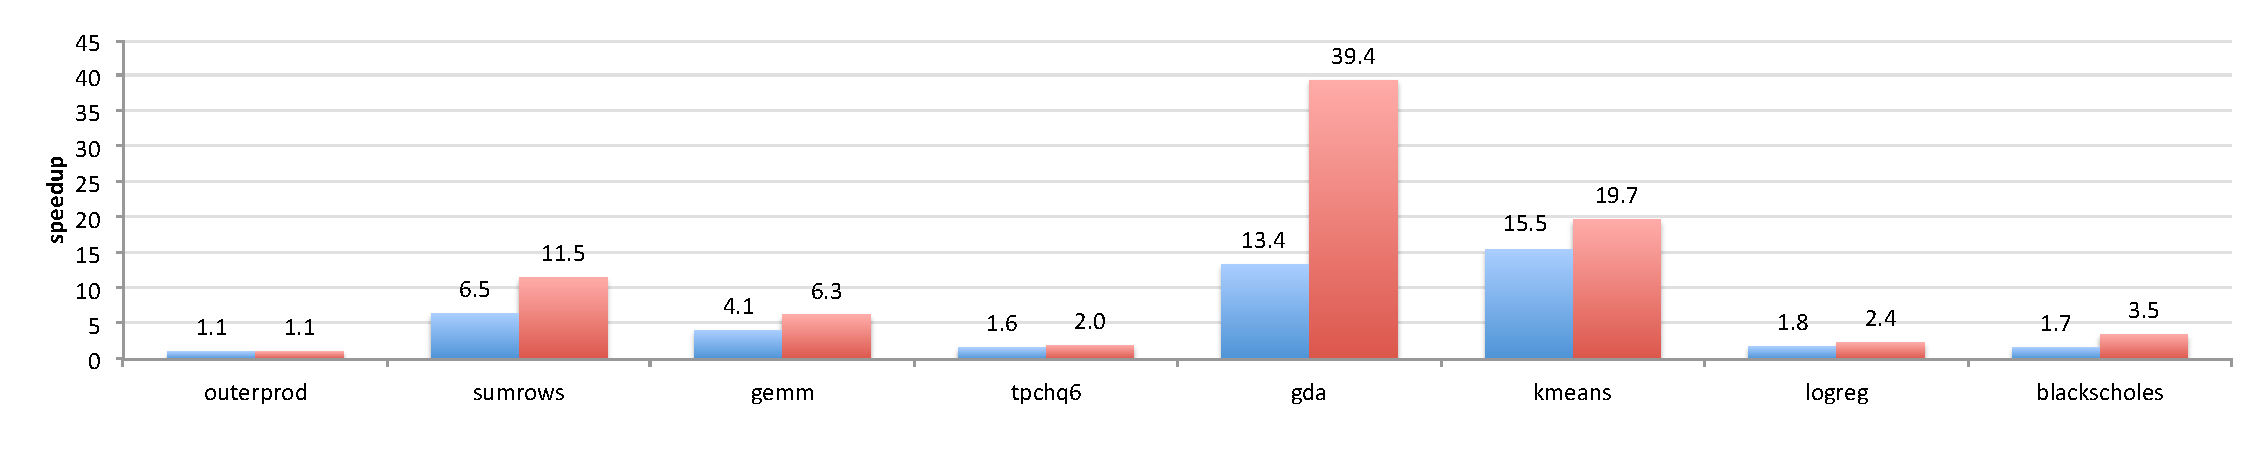
\includegraphics[width=\textwidth]{3-delite/figs/newspeedupbars1.pdf}
\vspace{10pt}
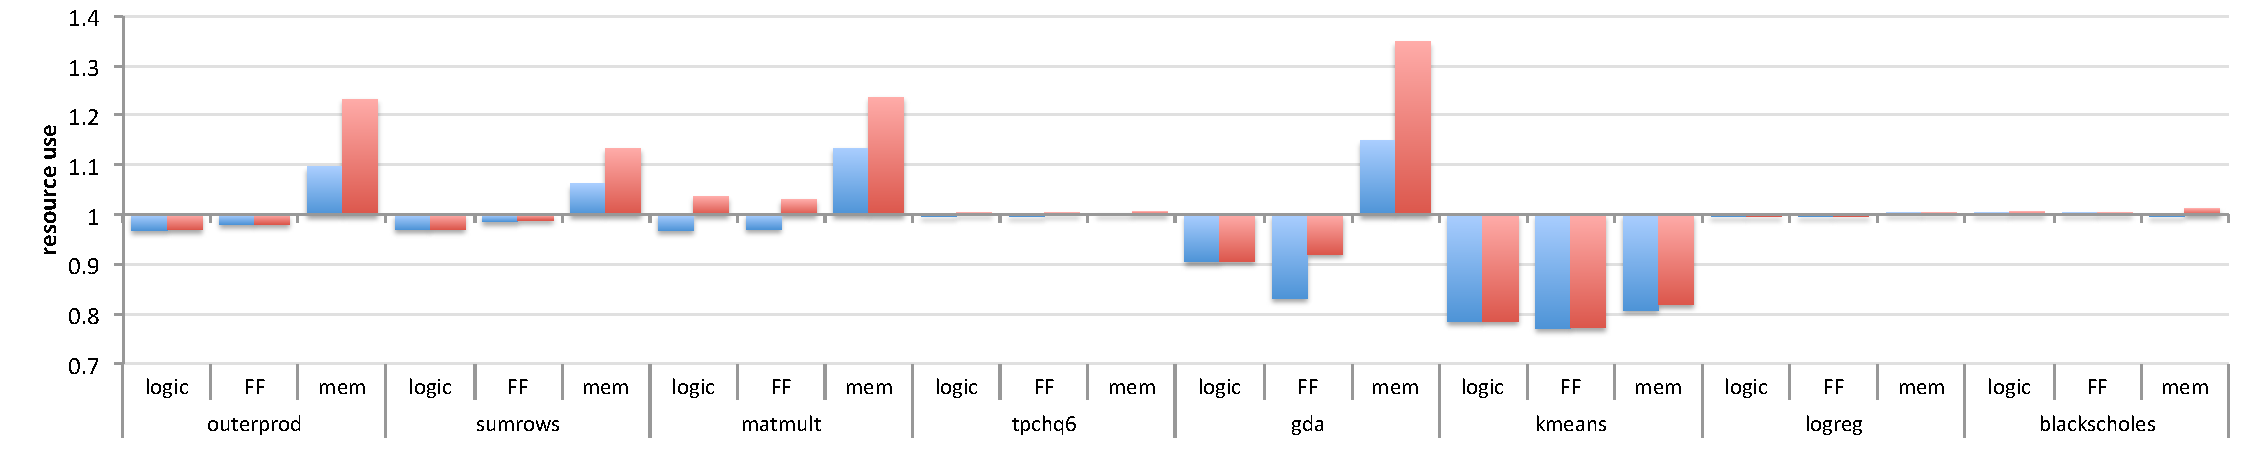
\includegraphics[width=\textwidth]{3-delite/figs/newspeedupbars2.pdf}

{
\fontfamily{phv}\selectfont
\footnotesize
\raisebox{-0.2em}{\tikz{\path[fill=bar1] (0,0) rectangle (1em,1em);}}
+tiling
\hspace{2em}
\raisebox{-0.2em}{\tikz{\path[fill=bar2] (0,0) rectangle (1em,1em);}}
+tiling+pipelining
}

\caption{Speedups and resource usages, relative to respective baseline designs, resulting from tiling and coarse-grained pipelining.}
\label{fig:speedup-bars}
\end{figure}

\paragraph{Impact of tiling alone}
Figure \ref{fig:speedup-bars} shows the obtained speedups as well as relative on-chip resource utilizations for each of the benchmarks.
Most benchmarks in our suite show significant speedup when tiling
transformations are enabled. Benchmarks like \emph{sumrows} and \emph{gemm}
benefit from inherent locality in their memory accesses. For \emph{gemm}, our automatically generated code
achieves a speedup of $4\times$ speedup over the baseline for a marginal increase of about $10\%$ on-chip memory usage.

Benchmarks \emph{outerprod} and \emph{tpchq6} do not
show a significant difference with our tiling transformations over the baseline.
This is because both \emph{outerprod} and
\emph{tpchq6} are both memory-bound benchmarks. \emph{Tpchq6} streams through the input once without reuse, and streaming
data input is already exploited in our baseline design. \emph{Blackscholes} has a similar data access pattern as \emph{tpchq6},
due to which it achieves a speedup similar to that of \emph{tpchq6}. Hence tiling does not provide any additional benefit.
Most of the locality in \emph{logreg} is already captured at burst-level granularity by our baseline. As a result, \emph{logreg}
achieves a modest speedup of $1.8x$ over the baseline due to tiling.
The core compute pipeline in \emph{outerprod} is memory-bound at the stage writing results to DRAM, which cannot be addressed
using tiling. Despite the futility of tiling in terms of performance, tiling \emph{outerprod}
has a noticeable increase in memory utilization as the intermediate result varies as the square of the tile size.

In \emph{kmeans} and \emph{gda}, some
of the input data structures are small enough that they can be held in on-chip memory. This completely
eliminates accesses to off-chip memory, leading to dramatic speedups of $13.4\times$ and $15.5\times$ respectively
with our tiling transformations. \emph{gda} uses more on-chip memory to store intermediate data. On the other hand, the tiled
version \emph{kmeans} utilizes less on-chip memory resources. This is because the baseline for \emph{kmeans} instantiates multiple
load and store units, each of which creates several control structures in order to read and write data from DRAM. Each of these control
structures includes address and data streams, which require several on-chip buffers. By tiling, we require a smaller number of load and store units.

\paragraph{Impact of coarse-grained pipelining}
The second speedup bar in Figure~\ref{fig:speedup-bars} shows the benefits of our pipelining analysis.
Coarse-grained pipelines increase throughput
at the expense of additional on-chip memory used for double buffers.
This overlaps design compute with data transfer and helps to hide the cost of the slower stage. Benchmarks like
\emph{gemm} and \emph{sumrows} naturally benefit from this coarse-grained pipelining because the memory transfer time is completely overlapped
with the compute, resulting in speedups of $6.3\times$ and $11.5\times$ respectively.
Pipelining also exploits overlap in
streaming benchmarks like \emph{tpchq6} and \emph{blackscholes}, where the input data is fetched and stored simultaneously with the core computation.

The speedup due to coarse-grained pipelining is largely determined by balancing between stages. Stages with roughly equal number of cycles benefit
the most, as this achieves the most overlap. Unbalanced stages are limited by the slowest stage, thus limiting performance.
We observe this behavior in \emph{outerprod},
where the pipeline is bottlenecked by the stage writing results back to DRAM.
The pipeline in \emph{logreg} is bottlenecked
at the stage performing dot products of all the points in the input tile with the \emph{theta} vector. As we only parallelize the
innermost parallel pattern in this work, only a single dot product is produced at a time, even though the dot product itself
is executed in parallel across the point dimensions. On the other hand, applications
like \emph{gda}, \emph{kmeans} and \emph{sumrows} greatly benefit from coarse-grained pipelining.
In particular, \emph{gda} naturally
maps to nested pipelines that are well-balanced.
The stage loading the input tile overlaps execution with the stage
computing the output tile and the stage storing the output tile. The stage computing the output tile is also
a pipeline where the stages perform vector subtraction, vector outer product and accumulation. We parallelize the vector
outer product stage as it is the most compute-heavy part of the algorithm; parallelizing the vector outer product enables
the pipeline to achieve greater throughput. This yields an overall speedup of $39.4\times$
over the baseline.

\section{Conclusion}

In this chapter, we introduced a series of compilation steps necessary to prepare
an intermediate representation composed of nested parallel patterns
for hardware compilation. We described a set of simple transformation
rules which can be used to automatically tile parallel patterns which exploit semantic information inherent within
these patterns and which place fewer restrictions on the program’s memory accesses than previous work. We then presented a simple analysis step for annotating pipelining information for
consumption by the lower level compiler. Finally, we presented experimental results
for a set of benchmarks in the machine learning and data
querying domains which show that these compilation steps
provide performance improvements of up to $39.4\times$ with a
minimal impact on FPGA resource usage.

